% chapter2.tex
% !TEX root = ../main.tex
\newpage
\begin{center}
    {\large\textbf{CHƯƠNG 2: PHÁC THẢO GIAO DIỆN}}\\
\end{center}

% Defining chapter and section
\section*{2.1 Tổng quan chương}
% Describing the introduction content
Sau khi hoàn tất quá trình khảo sát nhu cầu người dùng, phân tích các hệ thống hiện có và xác định các yêu cầu cơ bản, nhóm dự án tiến hành bước tiếp theo trong quy trình thiết kế: xây dựng các bản phác thảo giao diện cho hệ thống đặt vé xe khách liên tỉnh.

% Outlining objectives
Mục tiêu của chương này là trình bày chi tiết các bản phác thảo giao diện ban đầu, tạo nền tảng cho việc phát triển phiên bản thiết kế hoàn chỉnh. Các bản phác thảo được xây dựng dựa trên các cơ sở sau:
\begin{itemize}
    \item Nhu cầu thực tế thu thập từ quá trình khảo sát người dùng.
    \item Những điểm mạnh được phân tích từ các hệ thống đặt vé hiện hành.
    \item Các nguyên tắc thiết kế tương tác hiệu quả, tham khảo từ cuốn \textit{The Design of Everyday Things} của Don Norman.
\end{itemize}

% Explaining content structure and user flow
Chương này cũng làm rõ định hướng về cấu trúc nội dung, cách bố trí các thành phần chính trên từng trang giao diện, cũng như hành trình sử dụng của người dùng (user flow) trong hệ thống, đảm bảo tính trực quan và hiệu quả trong trải nghiệm người dùng.

% Defining section for website description
\section*{2.1 Tổng quan và Phân loại Giao diện Người dùng}
Dựa trên kết quả phân tích được từ \textbf{Chương 1} hệ thống đặt vé xe khách liên tỉnh bao gồm các giao diện chính như sau:
% Trang chủ
\subsection*{Trang chủ}
\textbf{Chức năng:}
\begin{itemize}
    \item Ô tìm kiếm chuyến xe nổi bật, bao gồm các trường: điểm đi, điểm đến, ngày giờ khởi hành, và số lượng vé.
    \item Banner quảng cáo hiển thị các ưu đãi, tuyến xe phổ biến, hoặc thông tin về nhà xe đối tác nổi bật.
    \item Hiển thị các đánh giá từ khách hàng hoặc danh sách các tuyến xe được yêu thích.
\end{itemize}
\textbf{Tối ưu hóa:} Giao diện thân thiện, thời gian tải trang nhanh, thiết kế responsive đảm bảo tương thích với thiết bị di động.\\
\textbf{Mục đích:} Thu hút người dùng và hỗ trợ tìm kiếm chuyến xe tức thì.

% Trang tìm kiếm và danh sách chuyến xe
\subsection*{Trang tìm kiếm và danh sách chuyến xe}
\textbf{Chức năng:}
\begin{itemize}
    \item Hiển thị danh sách chuyến xe dựa trên thông tin tìm kiếm: giờ khởi hành, giá vé, loại xe, và nhà xe.
    \item Bộ lọc nâng cao: giá vé, giờ khởi hành, loại xe (giường nằm, limousine), tiện ích (wifi, điều hòa).
    \item Sắp xếp kết quả theo giá, thời gian, hoặc đánh giá.
\end{itemize}
\textbf{Tối ưu hóa:} Tải kết quả tìm kiếm nhanh, nút ``Xem chi tiết'' rõ ràng và dễ nhấn.\\
\textbf{Mục đích:} Giúp người dùng dễ dàng so sánh và lựa chọn chuyến xe phù hợp.

% Trang chi tiết chuyến xe
\subsection*{Trang chi tiết chuyến xe}
\textbf{Chức năng:}
\begin{itemize}
    \item Cung cấp thông tin chi tiết: lộ trình, thời gian, điểm đón/trả, và tiện ích trên xe.
    \item Sơ đồ ghế ngồi tương tác, cho phép chọn ghế và hiển thị trạng thái ghế (trống/đã đặt).
    \item Hiển thị đánh giá và nhận xét từ khách hàng trước đó.
    \item Nút ``Đặt vé ngay'' và thông tin giá vé minh bạch.
\end{itemize}
\textbf{Tối ưu hóa:} Hiển thị hình ảnh thực tế của xe hoặc nhà xe (nếu có).\\
\textbf{Mục đích:} Cung cấp thông tin đầy đủ để người dùng đưa ra quyết định đặt vé.

% Trang đặt vé
\subsection*{Trang đặt vé}
\textbf{Chức năng:}
\begin{itemize}
    \item Form nhập thông tin hành khách: họ tên, số điện thoại, email, CMND/CCCD (nếu cần).
    \item Tùy chọn chọn ghế hoặc loại vé (nếu chưa chọn ghế trước đó).
    \item Hiển thị tóm tắt đơn hàng: thông tin chuyến, giá vé, số lượng vé.
    \item Tích hợp mã khuyến mãi (nếu có).
\end{itemize}
\textbf{Tối ưu hóa:} Form đơn giản, kiểm tra lỗi nhập liệu tức thời.\\
\textbf{Mục đích:} Thu thập thông tin hành khách nhanh chóng và chính xác.

% Trang thanh toán
\subsection*{Trang thanh toán}
\textbf{Chức năng:}
\begin{itemize}
    \item Hiển thị hóa đơn chi tiết: giá vé, phí dịch vụ, tổng cộng.
    \item Tích hợp các cổng thanh toán: thẻ ngân hàng, ví điện tử (Momo, ZaloPay), chuyển khoản, hoặc trả sau (nếu có).
    \item Xác nhận điều khoản sử dụng và chính sách hoàn vé.
\end{itemize}
\textbf{Tối ưu hóa:} Bảo mật cao (SSL, mã OTP), giao diện thanh toán rõ ràng và dễ sử dụng.\\
\textbf{Mục đích:} Đảm bảo giao dịch an toàn và thuận tiện.

% Trang xác nhận đặt vé
\subsection*{Trang xác nhận đặt vé}
\textbf{Chức năng:}
\begin{itemize}
    \item Hiển thị mã vé, thông tin chuyến (giờ, địa điểm), và thông tin hành khách.
    \item Tùy chọn gửi vé qua email, SMS, hoặc tải xuống dưới dạng PDF.
    \item Hướng dẫn kiểm tra vé hoặc liên hệ hỗ trợ nếu cần.
\end{itemize}
\textbf{Tối ưu hóa:} Gửi thông báo đẩy qua ứng dụng (nếu có) hoặc email tự động.\\
\textbf{Mục đích:} Xác nhận giao dịch thành công và cung cấp thông tin vé đầy đủ.

% Trang lịch sử vé và thông tin vé người dùng
\subsection*{Trang lịch sử vé và thông tin vé người dùng}
\textbf{Chức năng:}
\begin{itemize}
    \item Hiển thị danh sách các vé xe mà người dùng đã đặt, bao gồm thông tin chuyến đi (ngày giờ, tuyến xe, điểm đi, điểm đến).
    \item Cung cấp tính năng xem chi tiết vé, bao gồm thông tin về giá vé, trạng thái vé (đã thanh toán, chưa thanh toán, đã sử dụng).
    \item Cho phép người dùng tải lại vé điện tử hoặc in vé nếu cần.
    \item Cung cấp tính năng tìm kiếm và lọc theo các tiêu chí như ngày tháng, trạng thái vé, tuyến xe.
\end{itemize}
\textbf{Tối ưu hóa:} 
\begin{itemize}
    \item Tối ưu hóa giao diện người dùng (UI) để dễ dàng thao tác và truy cập thông tin.
    \item Tối ưu tốc độ tải trang, giảm thiểu độ trễ khi truy vấn lịch sử vé.
    \item Bảo mật thông tin người dùng, đảm bảo tính riêng tư và bảo mật dữ liệu cá nhân.
\end{itemize}
\textbf{Mục đích:} 
\begin{itemize}
    \item Giúp người dùng dễ dàng theo dõi và quản lý các vé xe đã mua.
    \item Cung cấp cho người dùng một công cụ quản lý vé tiện lợi, giúp họ kiểm tra và theo dõi trạng thái vé nhanh chóng.
    \item Tăng mức độ hài lòng của khách hàng thông qua việc cung cấp dịch vụ và thông tin minh bạch.
\end{itemize}


% Trang tài khoản người dùng
\subsection*{Trang tài khoản người dùng}
\textbf{Chức năng:}
\begin{itemize}
    \item Quản lý thông tin cá nhân: họ tên, email, số điện thoại, địa chỉ.
    \item Xem lịch sử đặt vé, trạng thái vé (đã đi, đang chờ, đã hủy).
    \item Tùy chọn lưu phương thức thanh toán hoặc đổi mật khẩu.
    \item Tích hợp đăng nhập qua Google/Facebook.
\end{itemize}
\textbf{Tối ưu hóa:} Giao diện đơn giản, bảo mật với hình thức otp không mật khẩu tạo trải nghiệm tốt.\\
\textbf{Mục đích:} Cá nhân hóa trải nghiệm và quản lý vé dễ dàng.

% Trang liên hệ
\subsection*{Trang liên hệ}
\textbf{Chức năng:}
\begin{itemize}
    \item Cung cấp thông tin liên hệ: hotline, email, mạng xã hội.
    \item Form gửi yêu cầu hỗ trợ (vấn đề về vé, thanh toán, hoặc khiếu nại).
    \item Tích hợp chatbot trực tuyến (nếu có).
\end{itemize}
\textbf{Tối ưu hóa:} Phản hồi nhanh qua email hoặc thông báo đẩy.\\
\textbf{Mục đích:} Hỗ trợ người dùng hiệu quả khi gặp vấn đề.

% Trang thông tin và FAQ
\subsection*{Trang thông tin và FAQ}
\textbf{Chức năng:}
\begin{itemize}
    \item Giới thiệu về công ty/dịch vụ, sứ mệnh, và tầm nhìn.
    \item FAQ giải đáp các thắc mắc về đặt vé, thanh toán, chính sách hoàn/hủy vé, và hành lý.
    \item Chính sách bảo mật và điều khoản sử dụng.
\end{itemize}
\textbf{Tối ưu hóa:} Nội dung rõ ràng, dễ tìm kiếm, hỗ trợ tối ưu hóa SEO.\\
\textbf{Mục đích:} Tăng độ tin cậy và giải đáp thắc mắc của người dùng.

% Trang ưu đãi/khuyến mãi
\subsection*{Trang ưu đãi/khuyến mãi}
\textbf{Chức năng:}
\begin{itemize}
    \item Hiển thị các chương trình giảm giá, mã khuyến mãi, hoặc combo vé.
    \item Kêu gọi hành động (CTA) để người dùng sử dụng mã ngay.
\end{itemize}
\textbf{Tối ưu hóa:} Cập nhật thường xuyên, tích hợp với email marketing.\\
\textbf{Mục đích:} Thu hút người dùng và tăng tỷ lệ đặt vé.

% Trang đánh giá nhà xe
\subsection*{Trang đánh giá nhà xe}
\textbf{Chức năng:}
\begin{itemize}
    \item Cho phép người dùng đọc hoặc để lại đánh giá về nhà xe và chất lượng dịch vụ.
    \item Hiển thị điểm đánh giá trung bình và các bình luận nổi bật.
\end{itemize}
\textbf{Tối ưu hóa:} Kiểm duyệt bình luận để tránh nội dung không phù hợp.\\
\textbf{Mục đích:} Tăng tính minh bạch và tạo niềm tin cho người dùng.

% Trang tin tức/blog
\subsection*{Trang tin tức/blog}
\textbf{Chức năng:}
\begin{itemize}
    \item Bài viết về du lịch, mẹo đi xe, hoặc thông tin về các tuyến xe mới.
    \item Tích hợp chia sẻ bài viết lên mạng xã hội.
\end{itemize}
\textbf{Tối ưu hóa:} Tối ưu SEO với từ khóa liên quan đến du lịch và đặt vé.\\
\textbf{Mục đích:} Tăng tương tác và thu hút lưu lượng truy cập.



% Trang lỗi
\subsection*{Trang lỗi}
\textbf{Chức năng:}
\begin{itemize}
    \item Hiển thị thông báo lỗi (404, 500, v.v.) với hướng dẫn quay lại trang chủ hoặc liên hệ hỗ trợ.
    \item Thiết kế thân thiện, có nút kêu gọi hành động (CTA) rõ ràng.
\end{itemize}
\textbf{Tối ưu hóa:} Giữ người dùng ở lại website thay vì thoát.\\
\textbf{Mục đích:} Cải thiện trải nghiệm người dùng khi gặp sự cố.\\

Để trình bày rõ hơn về cấu trúc giao diện, nhóm đã phân loại các trang theo chức năng và thiết bị sử dụng như được trình bày trong bảng sau:


\arrayrulecolor{lightblue}
\begin{longtable}{|
    >{\raggedright\arraybackslash}m{0.7cm}|
    >{\raggedright\arraybackslash}m{4cm}|
    >{\raggedright\arraybackslash}m{3cm}|
    >{\raggedright\arraybackslash}m{6cm}|
}
    \hline
    \rowcolor{lightblue}
    \textbf{STT} & \textbf{\ Tên trang} & \textbf{Loại thiết bị} & \textbf{Mục đích} \\
    \hline
    \hline
1 & Trang chủ & Web và Mobile & Thu hút người dùng và hỗ trợ tìm kiếm chuyến xe tức thì. \\
\hline
2 & Tìm kiếm và danh sách chuyến xe & Web và Mobile & Giúp người dùng so sánh và chọn chuyến xe phù hợp. \\
\hline
3 & Chi tiết chuyến xe & Web và Mobile & Cung cấp thông tin đầy đủ để quyết định đặt vé. \\
\hline
4 & Đặt vé & Web và Mobile & Thu thập thông tin hành khách nhanh chóng, chính xác. \\
\hline
5 & Thanh toán & Web và Mobile & Đảm bảo giao dịch an toàn và thuận tiện. \\
\hline
6 & Xác nhận đặt vé & Web và Mobile & Xác nhận giao dịch và cung cấp thông tin vé. \\
\hline
7 & Tài khoản người dùng & Web và Mobile & Cá nhân hóa trải nghiệm và quản lý vé dễ dàng. \\
\hline
8 & Liên hệ & Web và Mobile & Hỗ trợ người dùng hiệu quả khi gặp vấn đề. \\
\hline
9 & Thông tin và FAQ & Web và Mobile & Tăng độ tin cậy và giải đáp thắc mắc. \\
\hline
10 & Ưu đãi/khuyến mãi & Web và Mobile & Thu hút người dùng và tăng tỷ lệ đặt vé. \\
\hline
11 & Đánh giá nhà xe & Web và Mobile & Tăng tính minh bạch và tạo niềm tin. \\
\hline
12 & Tin tức/blog & Web và Mobile & Tăng tương tác và thu hút lưu lượng truy cập. \\
\hline
14 & Trang lỗi & Web và Mobile & Cải thiện trải nghiệm người dùng khi gặp sự cố. \\
\hline
\caption{\textit{Bảng thông tin các trang giao diện chính.}}
\label{table4}
\end{longtable}
\section*{2.2 Luồng tương tác người dùng với hệ thống}


% Describing the purpose of the flowchart
Để đảm bảo trải nghiệm người dùng mượt mà, trực quan và dễ sử dụng trong hệ thống đặt vé xe khách, nhóm đã thiết kế một sơ đồ luồng (flowchart) chi tiết, mô tả toàn bộ quá trình tương tác giữa người dùng và hệ thống, từ khi truy cập vào hệ thống đến khi hoàn tất giao dịch đặt vé.

% Explaining the flowchart's role
Sơ đồ này cung cấp cái nhìn tổng quan, rõ ràng về các bước xử lý, cách tổ chức giao diện người dùng, và sự chuyển đổi mượt mà giữa các màn hình. Đồng thời, việc phân tách rõ ràng giữa các thao tác của người dùng, giao diện hệ thống, và quy trình xử lý backend đảm bảo tính nhất quán trong thiết kế, đồng thời hỗ trợ hiệu quả cho quá trình phát triển và bảo trì hệ thống.

% Defining color conventions
\subsection*{Quy ước màu sắc trong sơ đồ:}
\begin{itemize}
    \item \textcolor{blue}{\textbf{Màu xanh dương}}: Đại diện cho các hành động hoặc thao tác do người dùng thực hiện.
    \item \textcolor{orange}{\textbf{Màu cam}}: Biểu thị các màn hình giao diện được hiển thị trên hệ thống.
    \item \textcolor{green}{\textbf{Màu xanh lá cây}}: Chỉ các bước xử lý nội bộ (backend hoặc xử lý nội tuyến).
\end{itemize}

% Describing the flowchart process
\subsection*{Mô tả chi tiết luồng xử lý giao diện:}
\begin{enumerate}
    \item Người dùng truy cập \textbf{trang chủ} của hệ thống và thực hiện thao tác tìm kiếm chuyến xe dựa trên các tiêu chí như điểm đi, điểm đến, và thời gian.
    \item Hệ thống hiển thị \textbf{danh sách các chuyến xe phù hợp}. Người dùng chọn một chuyến xe cụ thể để xem thông tin chi tiết.
    \item Giao diện chuyển sang \textbf{trang chi tiết chuyến xe}, bao gồm sơ đồ ghế ngồi. Người dùng chọn ghế và số lượng vé mong muốn, sau đó nhấn nút xác nhận để tiếp tục.
    \item Nếu người dùng chưa đăng nhập, hệ thống hiển thị \textbf{màn hình xác thực tài khoản} (cho phép đăng nhập hoặc đăng ký tài khoản ngay tại bước này).
    \item Sau khi đăng nhập thành công, người dùng được chuyển đến \textbf{trang nhập thông tin hành khách} và chọn phương thức thanh toán.
    \item Hệ thống thực hiện \textbf{quy trình xử lý thanh toán} (backend). 
    \begin{itemize}
        \item Nếu thanh toán thành công, hệ thống hiển thị \textbf{màn hình xác nhận vé} với thông tin chi tiết về vé, hoàn tất quy trình đặt vé.
        \item Nếu thanh toán không thành công, hệ thống quay lại \textbf{bước chọn phương thức thanh toán}, cho phép người dùng thử lại với phương thức khác.
    \end{itemize}
\end{enumerate}

% Summarizing the flowchart's benefits
Sơ đồ luồng này đảm bảo mọi tương tác giữa người dùng và hệ thống được thực hiện một cách logic, minh bạch và hiệu quả, đồng thời hỗ trợ nhóm phát triển trong việc tối ưu hóa giao diện và chức năng của hệ thống.

% Placeholder for the flowchart image
\subsection*{Hình ảnh sơ đồ luồng xử lý giao diện:}
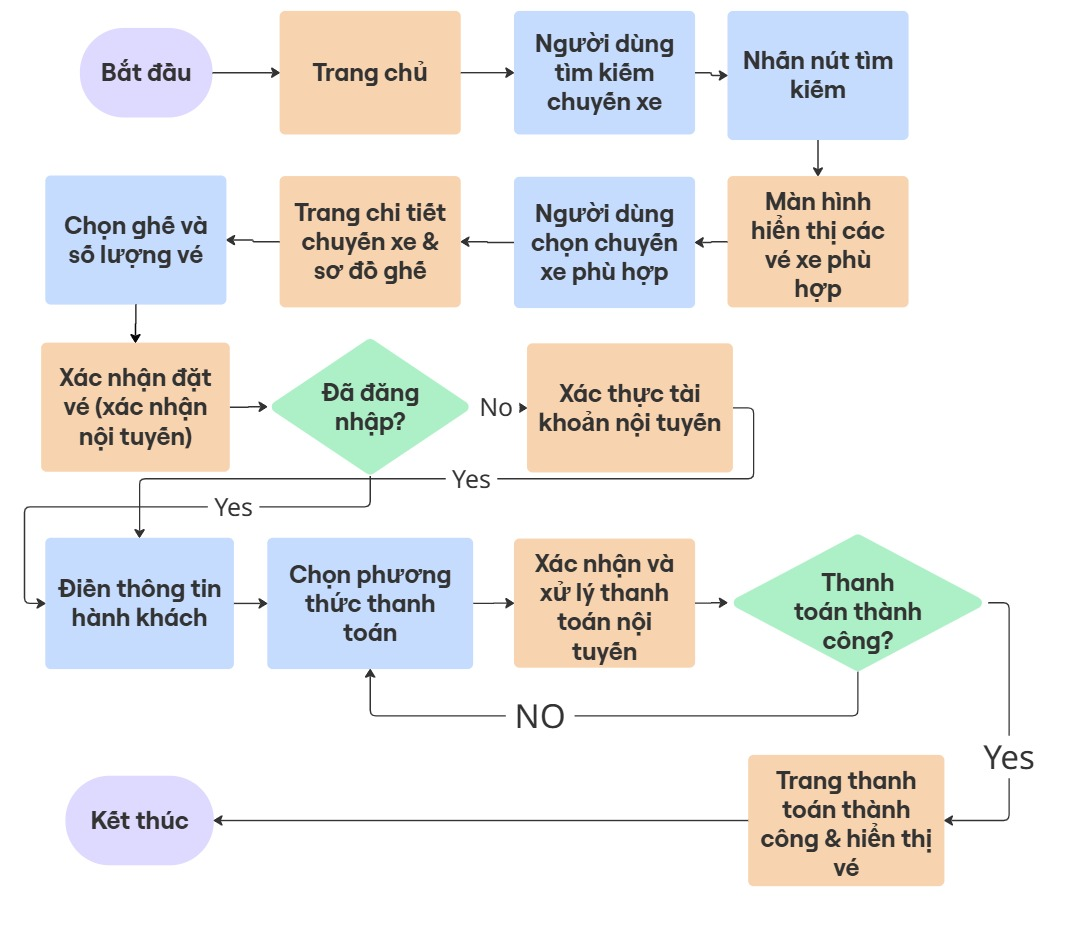
\includegraphics[width=\textwidth]{assets/chart/user_flow.jpg}
\begin{center}
    \textit{Hình 2.2: Sơ đồ luồng xử lý giao diện}
\end{center}

\section*{2.4. Phác thảo giao diện người dùng}

% Describing the wireframe development process
Sau khi xác định rõ các bước xử lý và luồng tương tác, nhóm đã tiến hành xây dựng wireframe (bản phác thảo khung giao diện) cho các màn hình chính của ứng dụng. Mục tiêu của bước này là xác định rõ ràng vị trí và thứ tự ưu tiên của các thành phần giao diện như ô tìm kiếm, danh sách chuyến xe, thông tin hành khách, nút thao tác,..., nhằm cung cấp cho nhóm phát triển một cái nhìn trực quan và thống nhất trước khi chuyển sang giai đoạn thiết kế chi tiết (hi-fi prototype).